\section{1 ARM}

\subsection{架构}

\begin{figure}[h]
  \centering
  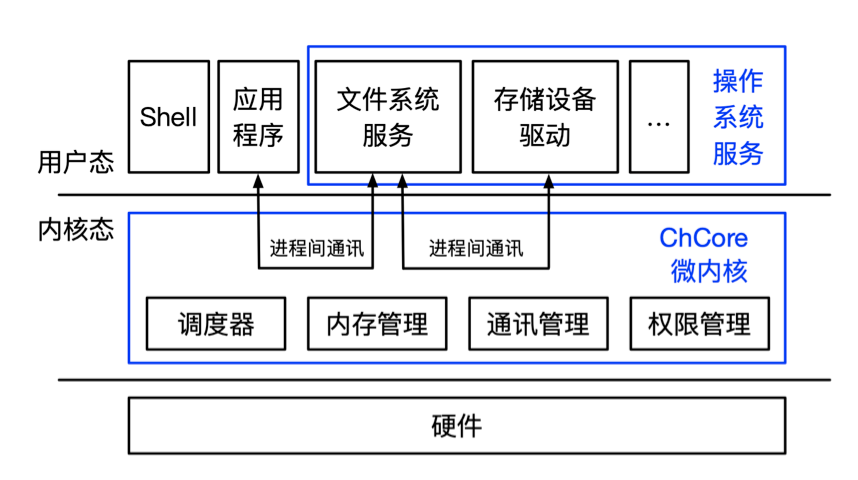
\includegraphics[width=0.2\textwidth]{imgs/chcore.png}
\end{figure}

ARM: 以手机处理器发家,CISC,简化的指令集,更少的历史包袱,更高级的抽象。

寄存器:31 个 64 位通用寄存器,X0 至 X30;1 个 PC 寄存器,4 个栈寄存器(切换异常等级时时保存 SP)SP-EL0 至 SP-EL3;3 个异常链接寄存器(保存异常的返回地址)ELR-EL1 至 ELR-EL3。不存在 ELR-EL0,因为不存在异常等级 0 下的异常处理器。